%!TEX root = ../thesis.tex
%*******************************************************************************
%********************************* Seventh Chapter *****************************
%*******************************************************************************
\cleardoublepage
\chapter{Application to wind turbine fatigue reliability and robustness}
\label{chpt:7}
%*******************************************************************************
\hfill
\localtableofcontents
\newpage

On risk levels for OWT: https://onlinelibrary.wiley.com/doi/epdf/10.1002/we.2610


%============================================================%
%============================================================%
\section{Introduction}
%============================================================%
%============================================================%
\begin{itemize}
    \item Recall the system random variables
    \item Define our quantity of interest
    \item recall the calculation on the damage and the linearity of Miner's 
    \item Expression of the failure probability (all in integral form)
\end{itemize}




%============================================================%
%============================================================%
\section{Surrogate modeling for reliability analysis}
%============================================================%
%============================================================%

%============================================================%
\subsection{High-performance computer evaluation}
%============================================================%

\begin{itemize}
    \item A specific wrapper was built with a double loop structure
    \item The design of experience in the X space is with a size 200
    \item This design is repeated for 11 identical seeds
    \item Altogether : 2200 DIEGO simulations for each evaluation in the Z space
    \item The current setup and the HPC facility CRONOS allows us to compute these 2200 simulations fully in parallel.
\end{itemize}

%============================================================%
\subsection{Design of experiments}
%============================================================%

\begin{itemize}
    \item The DoE concerns only two variables. The others intervene in the post-processing of DIEGO. 
    \item A Halton sequence with size 30 was first built. In 2D, it was the iterative design of experiments with the lowest discrepancy (among Halton, Sobol, KH, SP).
    \item After visualizing the first 30 points, an enrichment by KH is realized on an zone defined apriori.  
    \item This composite DoE has a final size of 50 points which represents in total more that 100k DIEGO simulations (each representing 45min of CPU time with this discretization timestep).
\end{itemize}

\begin{figure}
    \centering
    \begin{subfigure}{0.48\linewidth}
        \vskip -30pt
        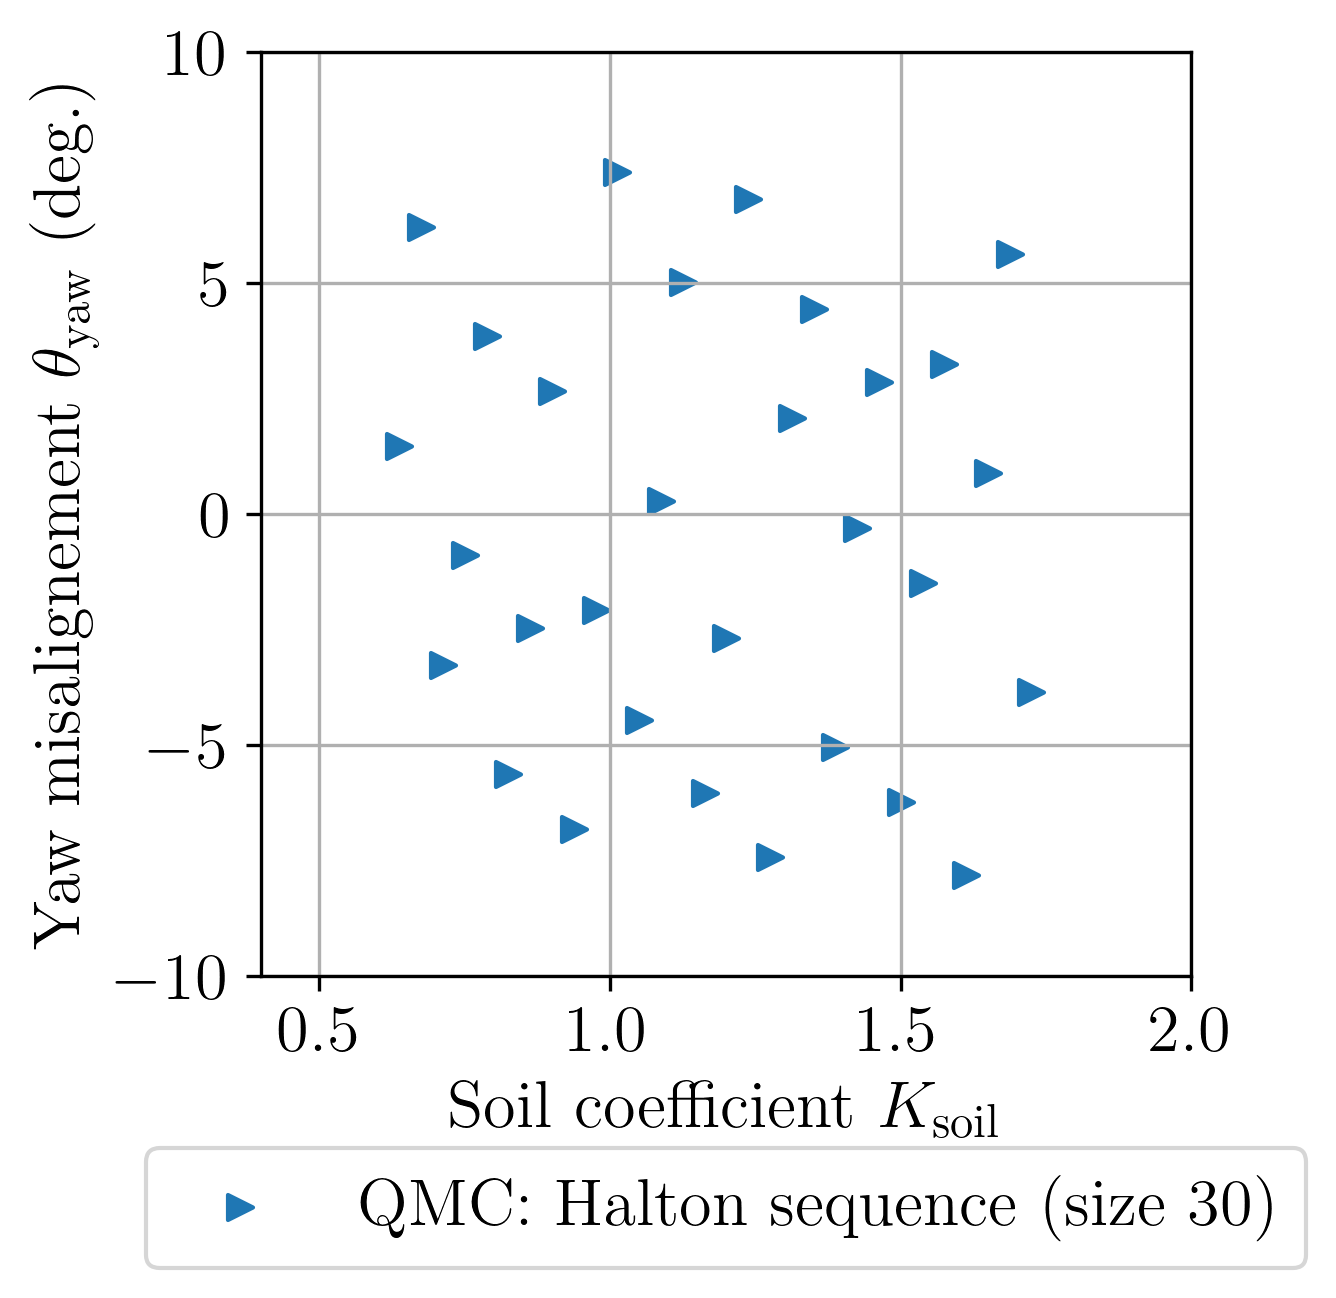
\includegraphics[width=\linewidth]{./part3/figures/OWT/initial_halton.png}
        \caption{Todo.}
    \end{subfigure}
    \begin{subfigure}{0.48\linewidth}
        %\vskip 0pt
        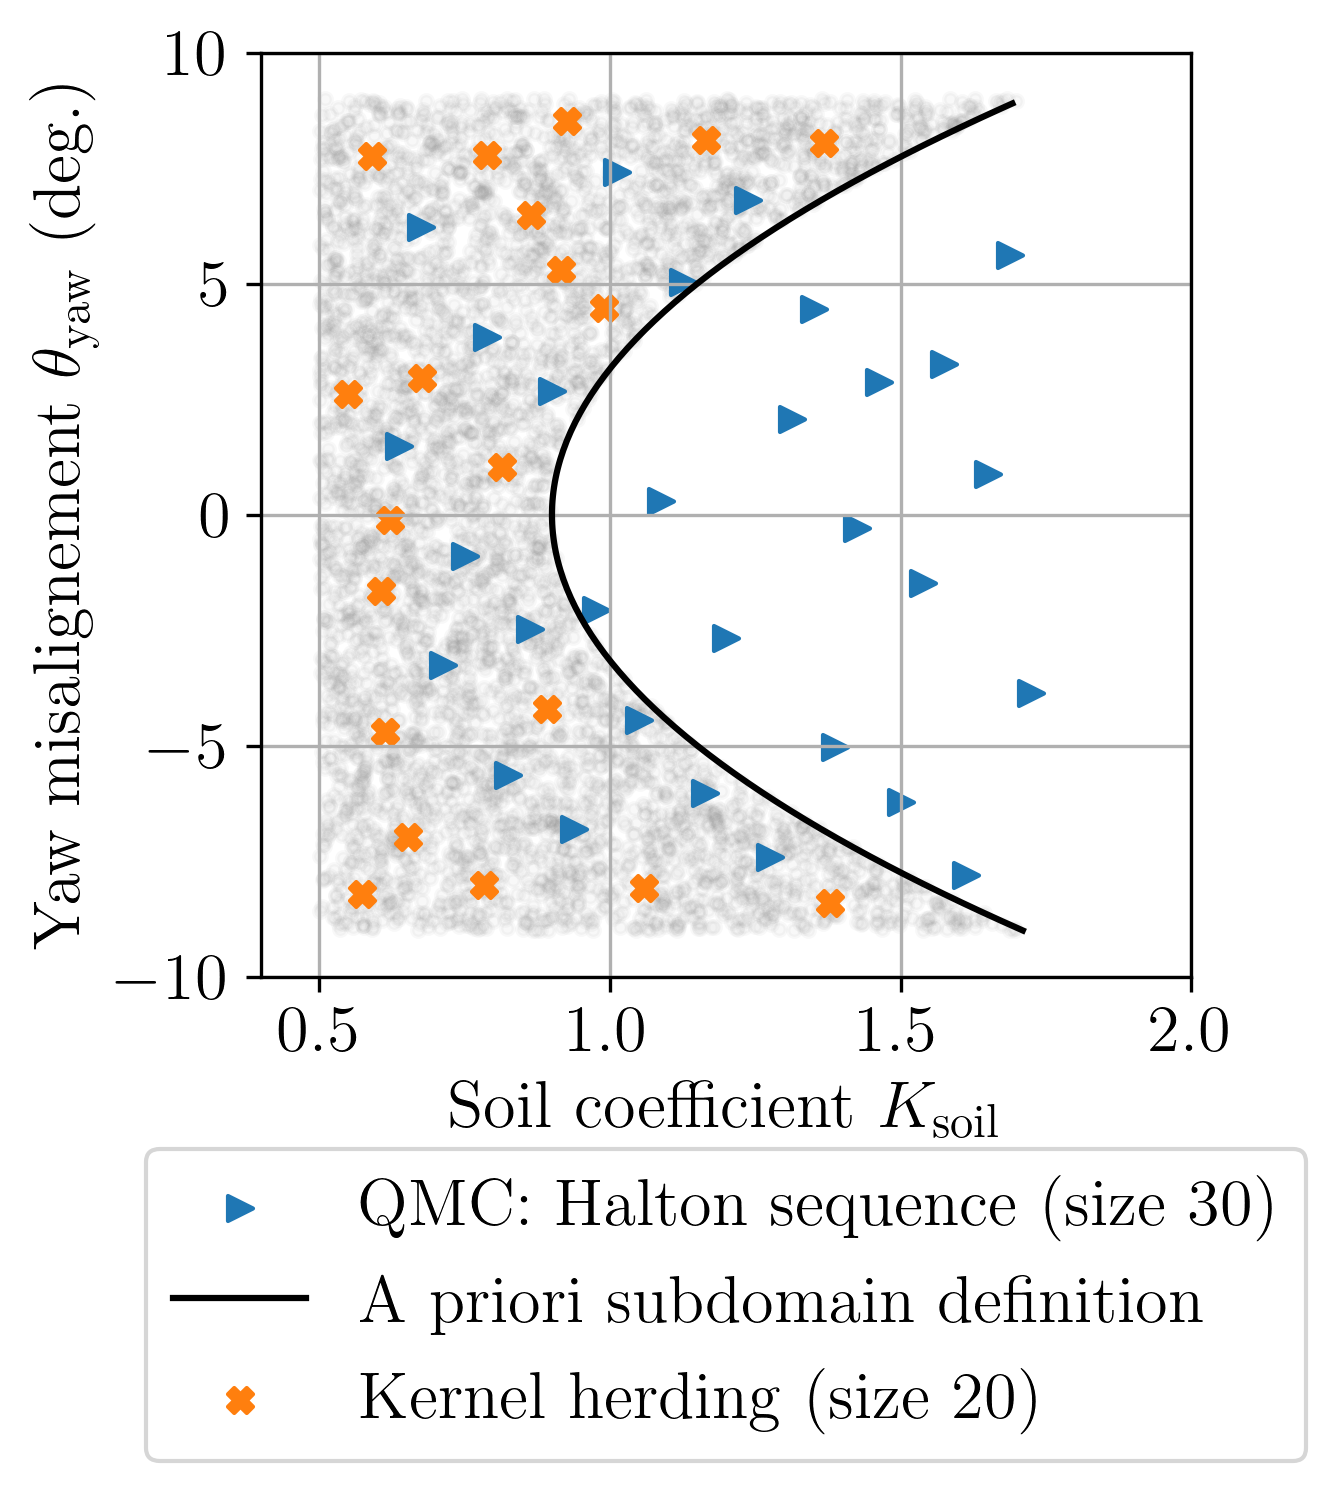
\includegraphics[width=\linewidth]{./part3/figures/OWT/initial_composite.png}
        \caption{Todo.}
    \end{subfigure}
    \label{fig:inital_doe}
    \caption{Todo.}
\end{figure}

\begin{figure}
    \centering
    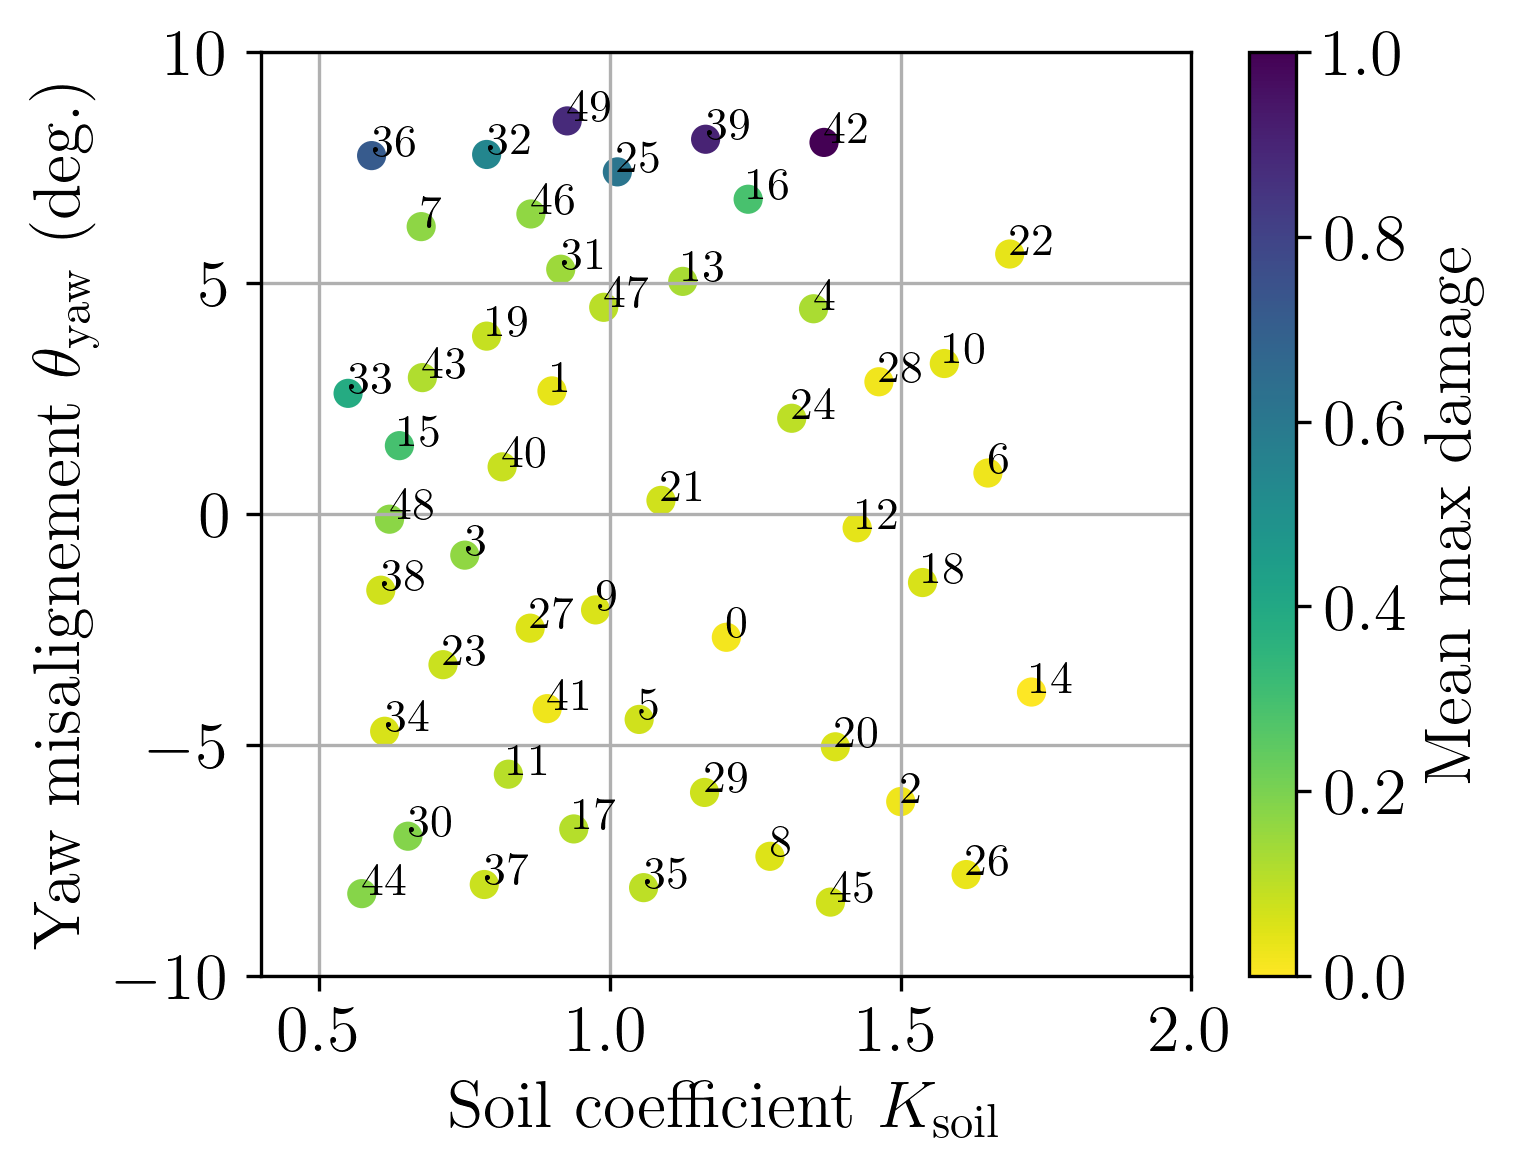
\includegraphics[width=0.6\linewidth]{./part3/figures/OWT/normalized_results_mean.png}
    \label{fig:evaluated_doe}
    \caption{Todo.}
\end{figure}


%============================================================%
\subsection{Gaussian process regression}
%============================================================%
\begin{itemize}
    \item Optimization of the hyperparameters by multi-start process in OT 
    \item Choice of kernel Matérn 5/2
    \item Why not adaptive? Because the reliability analysis happens at the borders of the domain. The quality of the GP in these areas is garanteed by the enrichement. Also: the enrichement might not be as robust to noisy functions. 
    \item LOO validation 
    \item Possible lack of trust in the mean estimation
\end{itemize}



\begin{figure}
    \centering
    \begin{subfigure}[b]{0.48\linewidth}
        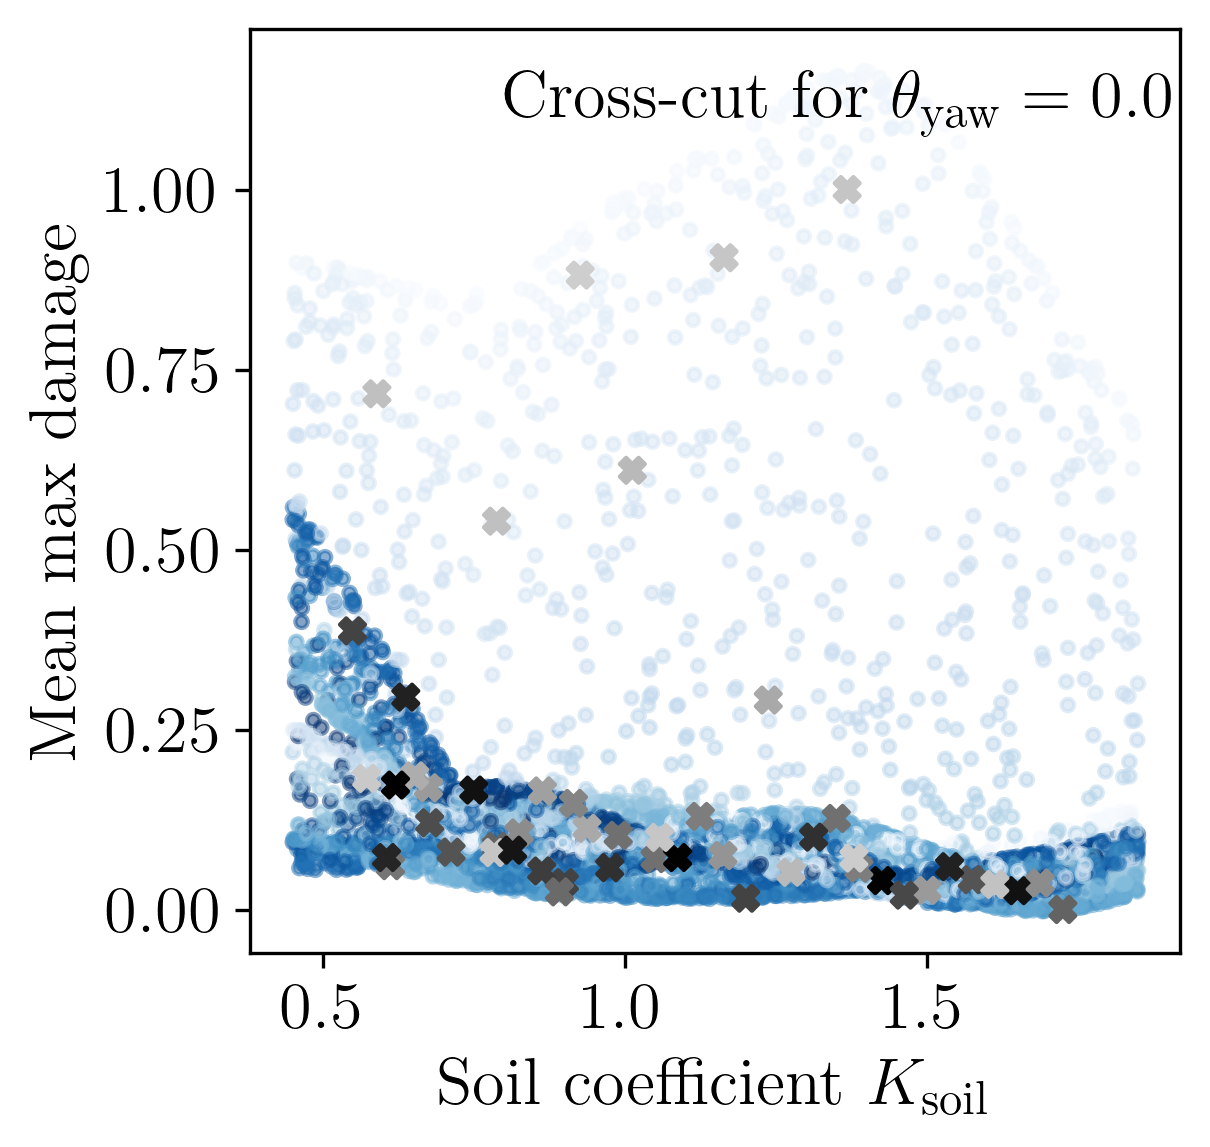
\includegraphics[width=\linewidth]{./part3/figures/OWT/dam_vs_soil_surrogate.png}
        \caption{Todo.}
    \end{subfigure}
    \begin{subfigure}[b]{0.48\linewidth}
        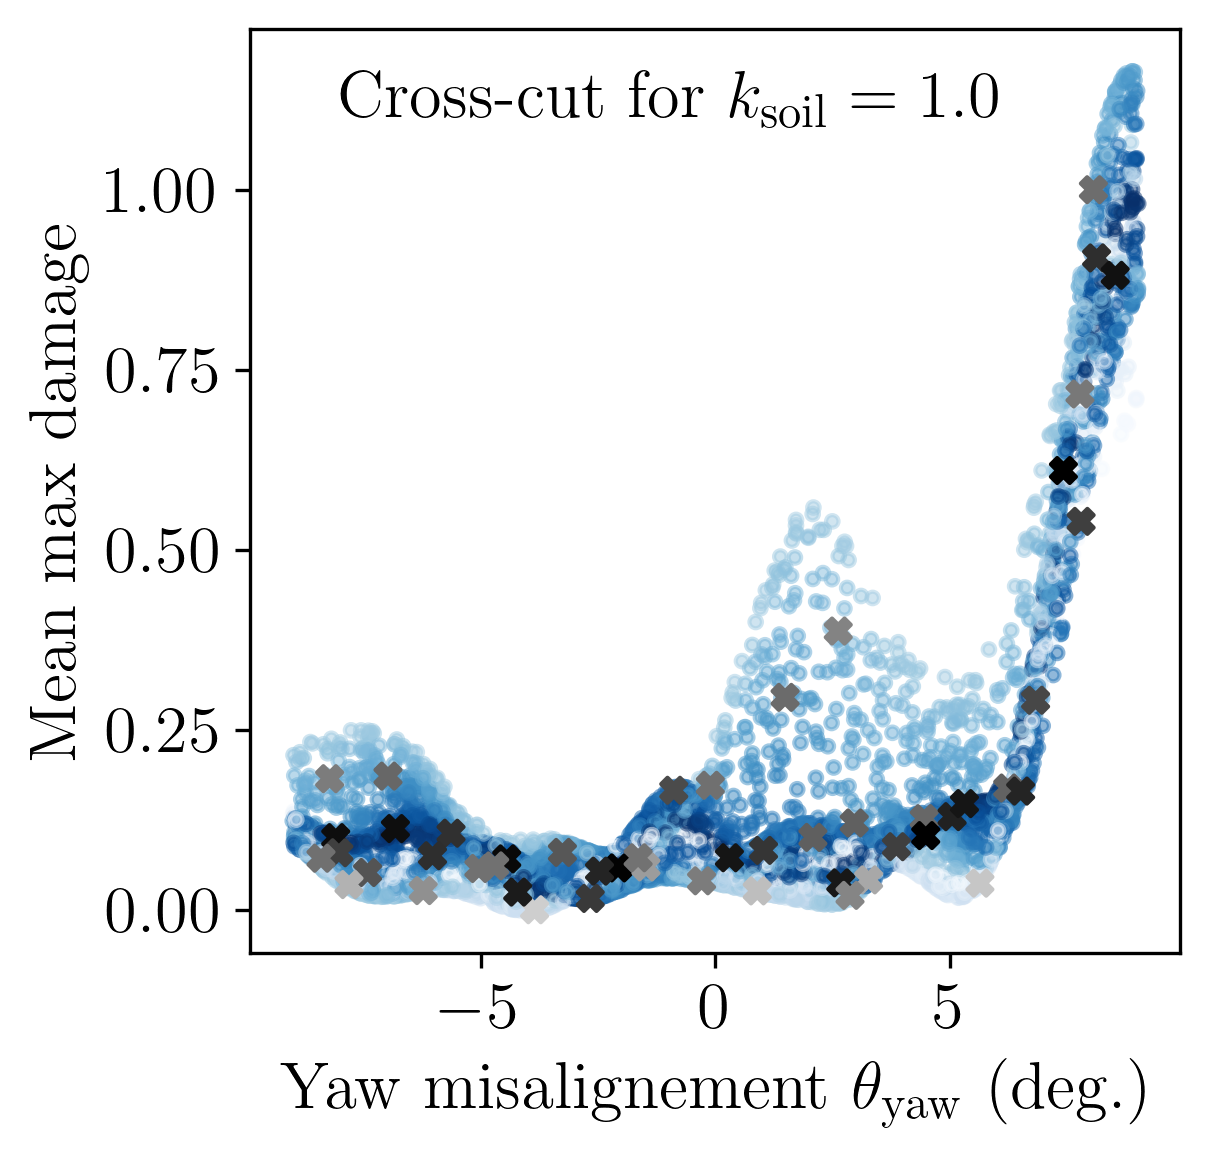
\includegraphics[width=\linewidth]{./part3/figures/OWT/dam_vs_yaw_surrogate.png}
        \caption{Todo.}
    \end{subfigure}
    \label{fig:owt_surrogate}
    \caption{Todo.}
\end{figure}

\begin{figure}
    \centering
    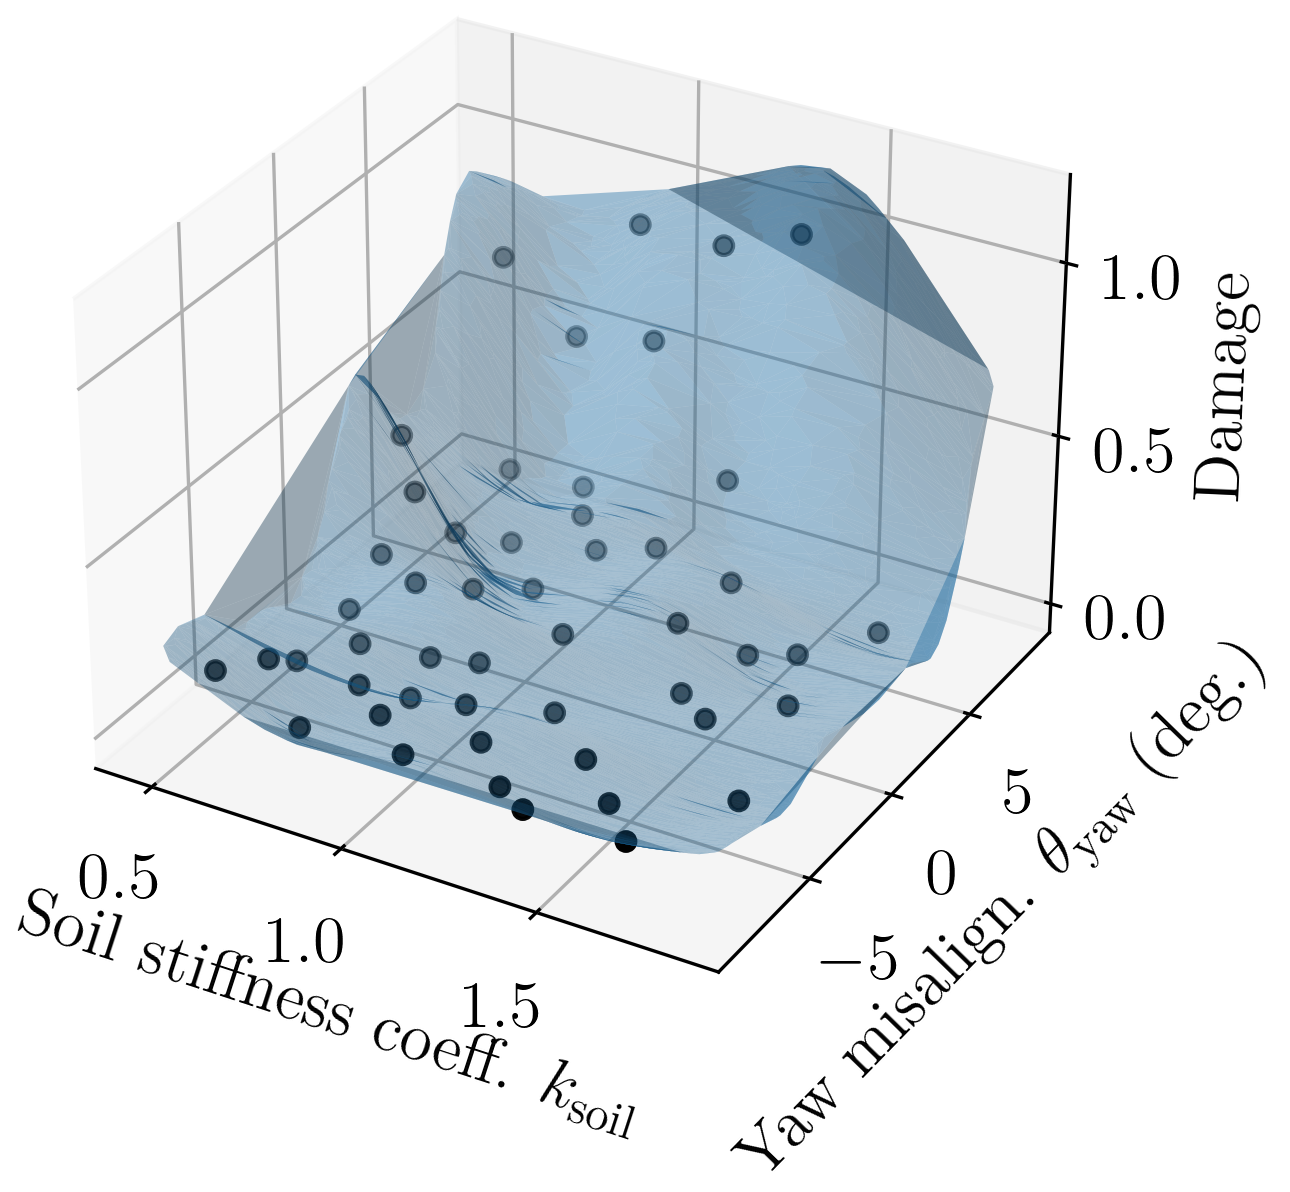
\includegraphics[width=0.7\linewidth]{./part3/figures/OWT/3D_surrogate.png}
    \label{fig:3d_owt_surrogte}
    \caption{Todo.}
\end{figure}

\begin{figure}
    \centering
    \begin{subfigure}[t]{0.42\linewidth}
        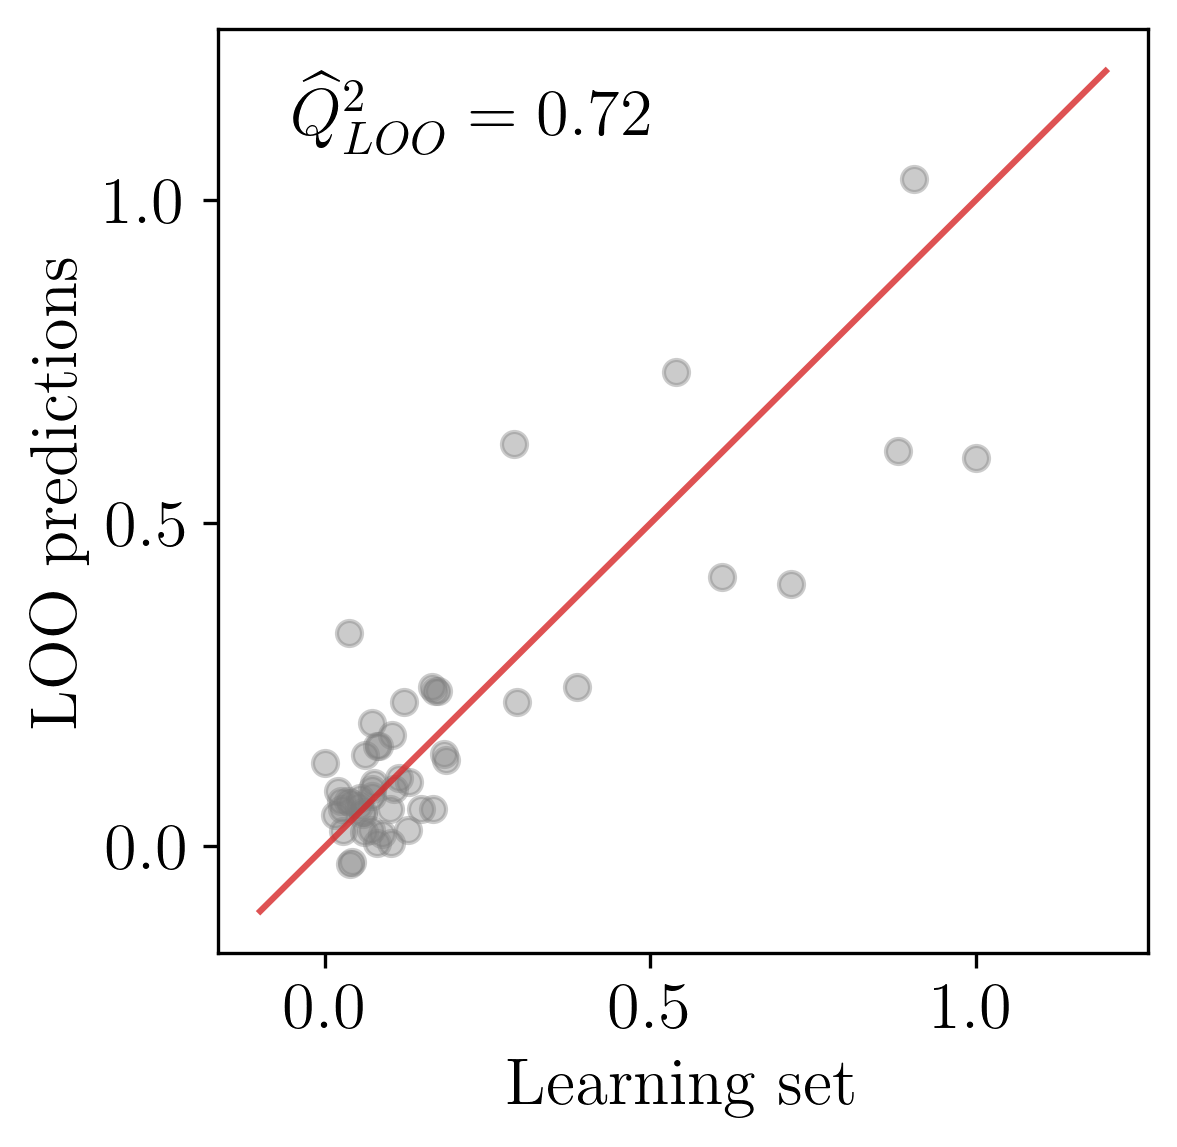
\includegraphics[width=\linewidth]{./part3/figures/OWT/loo_qqplot.png}
        \caption{Todo.}
    \end{subfigure}
    \begin{subfigure}[t]{0.55\linewidth}
        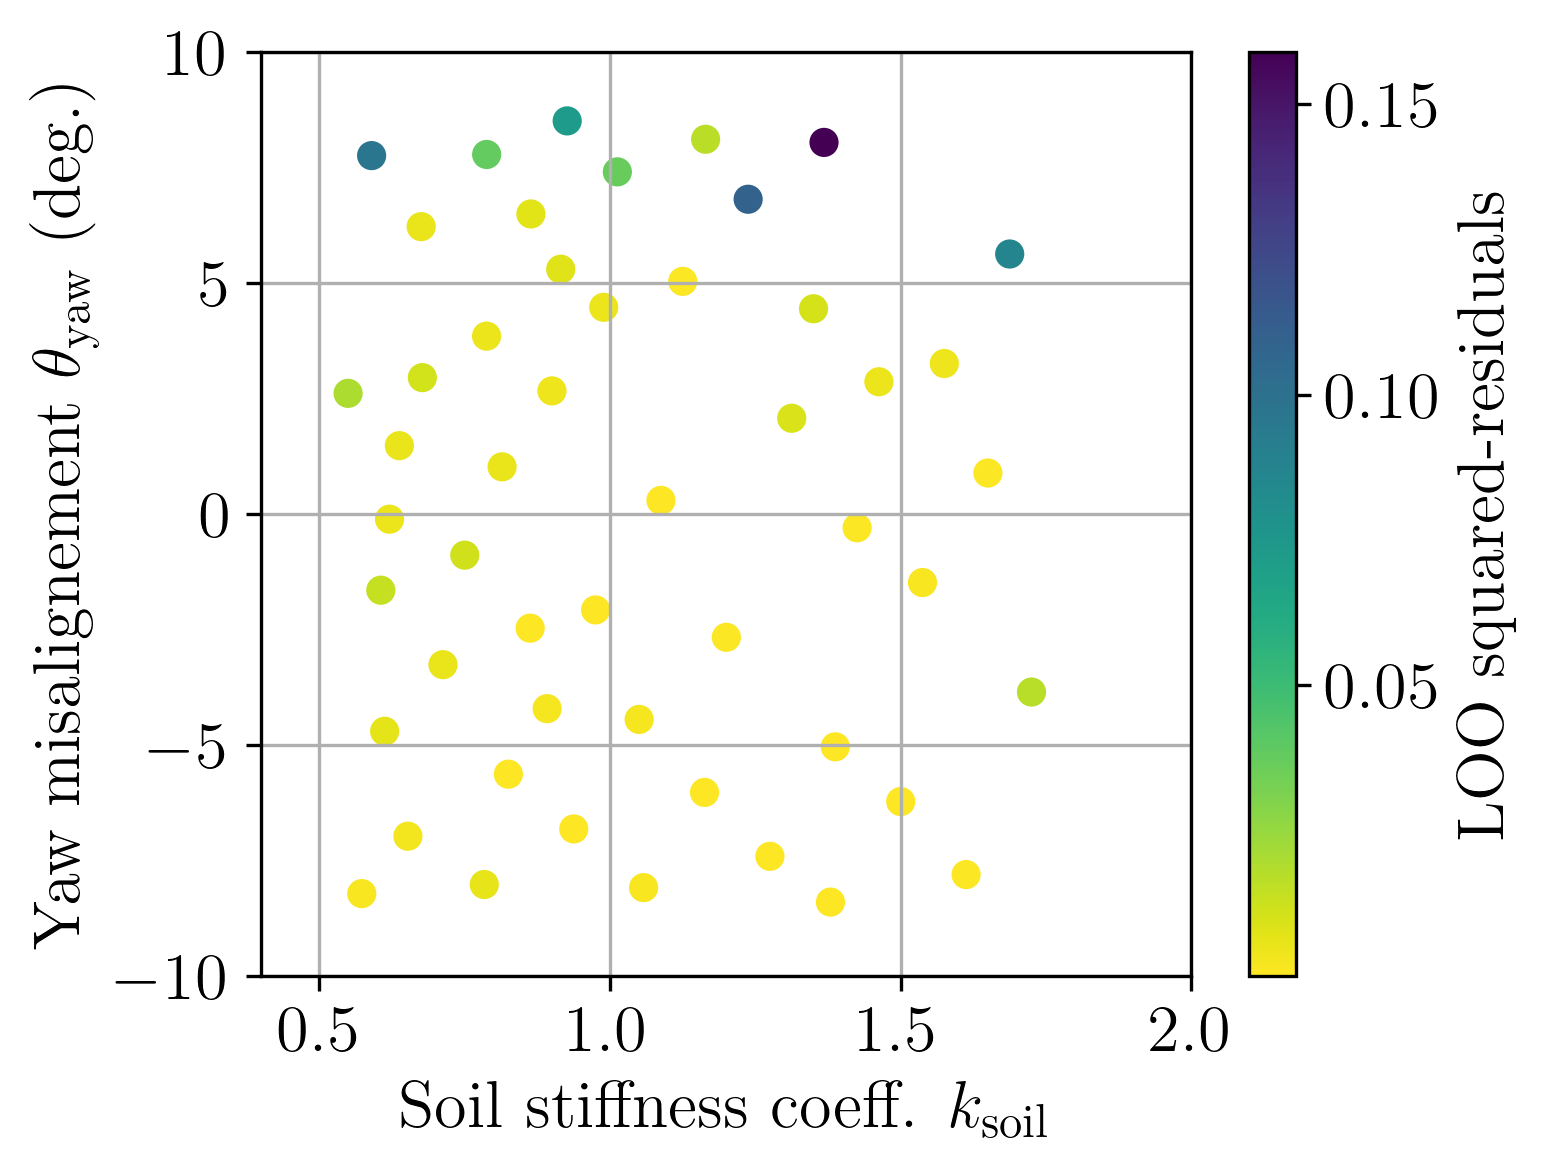
\includegraphics[width=\linewidth]{./part3/figures/OWT/loo_squared_res.png}
        \caption{Todo.}
    \end{subfigure}
    \label{fig:loo_validation}
    \caption{Todo.}
\end{figure}

%============================================================%
%============================================================%
\section{Reliability and robustness analysis}
%============================================================%
%============================================================%


%============================================================%
\subsection{Nominal reliability analysis}
%============================================================%
\begin{itemize}
    \item Nominal reliability analysis for 3 possible hypothesis of $D_cr$ and using multiple RA methods including BANCS
\end{itemize}


\begin{table*}[h]
    \centering
    \caption{Results of the numerical experiments (subset sample size $N=10^4$, $p_0=0.1$).}
    \begin{tabular}{l||c|c|c|c}
              &  \multicolumn{2}{c|}{$D_{\mathrm{cr}} \sim $ \bf Lognormal} & \multicolumn{2}{c}{$D_{\mathrm{cr}} \sim $ \bf Normal}\\
    \hline
    \bf RA method & $\widehat{\pf}$       & $\widehat{\mathrm{cov}}$    & $\widehat{\pf}$       & $\widehat{\mathrm{cov}}$ \\
    \hline\hline
    FORM      & $9.87 \times 10^{-13}$ & --                    & $3.35 \times 10^{-6}$ & --\\
    \hline
    FORM-IS   & $9.84 \times 10^{-13}$ & $1 \%$                & $3.36 \times 10^{-6}$ & $1 \%$\\
    \hline
    SS        & $9.46 \times 10^{-13}$ & $7 \%$               & $3.50 \times 10^{-6}$ & $4 \%$\\ 
    \end{tabular}
    \label{tab:result_table}
\end{table*}


%============================================================%
\subsection{Robustness analysis using the perturbed-law sensitivity indices}
%============================================================%
\begin{itemize}
    \item Definition of the PLI
    \item Perturbation protocol (only on the variance)
    \item Numerical results and discussion on the relevance of the study  
    \item Turbines are stopped about 6pc of their lifetime, which reduces the aerodynamic amortissement and therefore increases fatigue
    \item Starts and stops increase the damage
    \item Installation of the foundation can create early damage
\end{itemize}


\begin{figure}
    \centering
    \begin{subfigure}[t]{0.48\linewidth}
        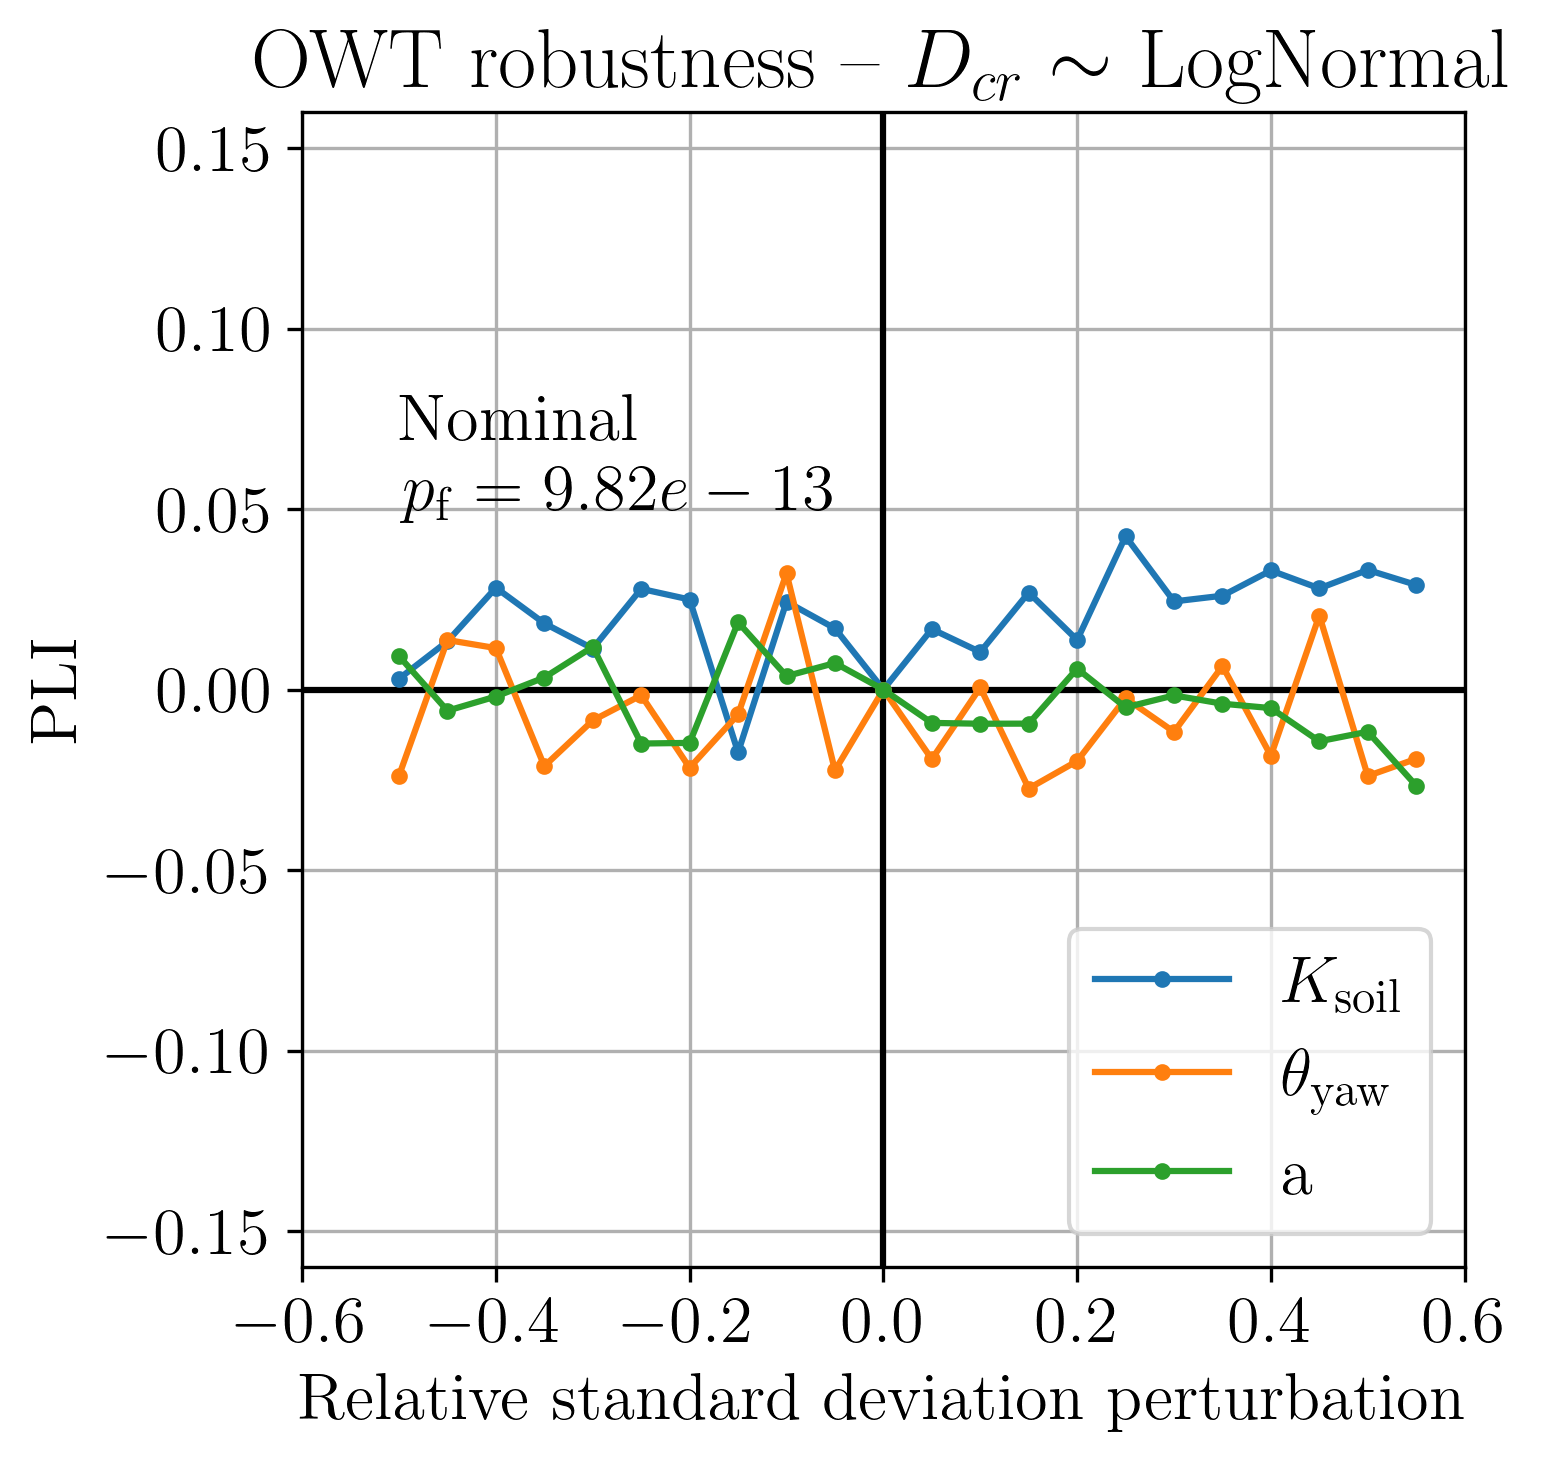
\includegraphics[width=\linewidth]{./part3/figures/OWT/PLI_ALL_Hyp_LogNormal.png}
        \caption{Todo.}
    \end{subfigure}
    \begin{subfigure}[t]{0.48\linewidth}
        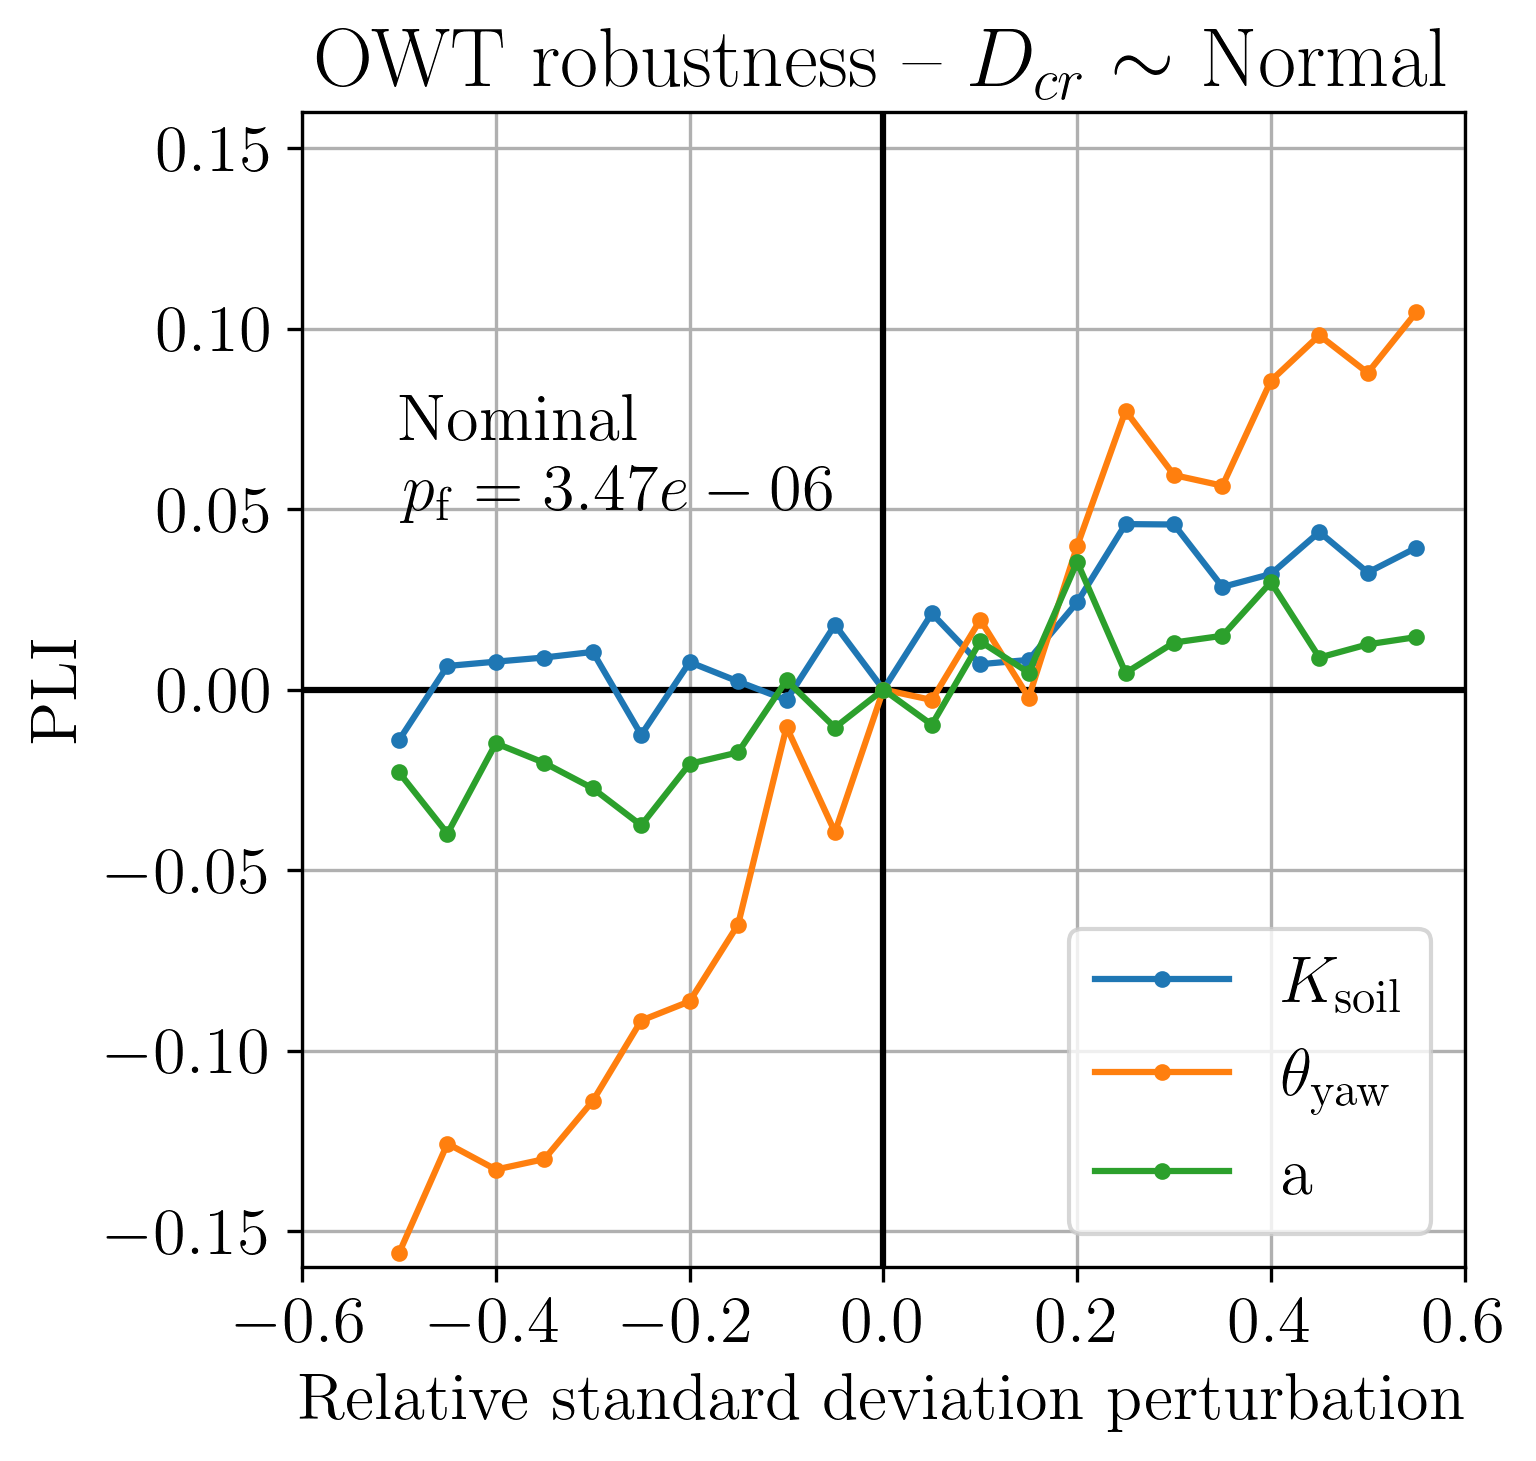
\includegraphics[width=\linewidth]{./part3/figures/OWT/PLI_ALL_Hyp_Normal.png}
        \caption{Todo.}
    \end{subfigure}
    \label{fig:pli_all}
    \caption{Todo.}
\end{figure}


\begin{figure}
    \centering
    \begin{subfigure}[t]{0.48\linewidth}
        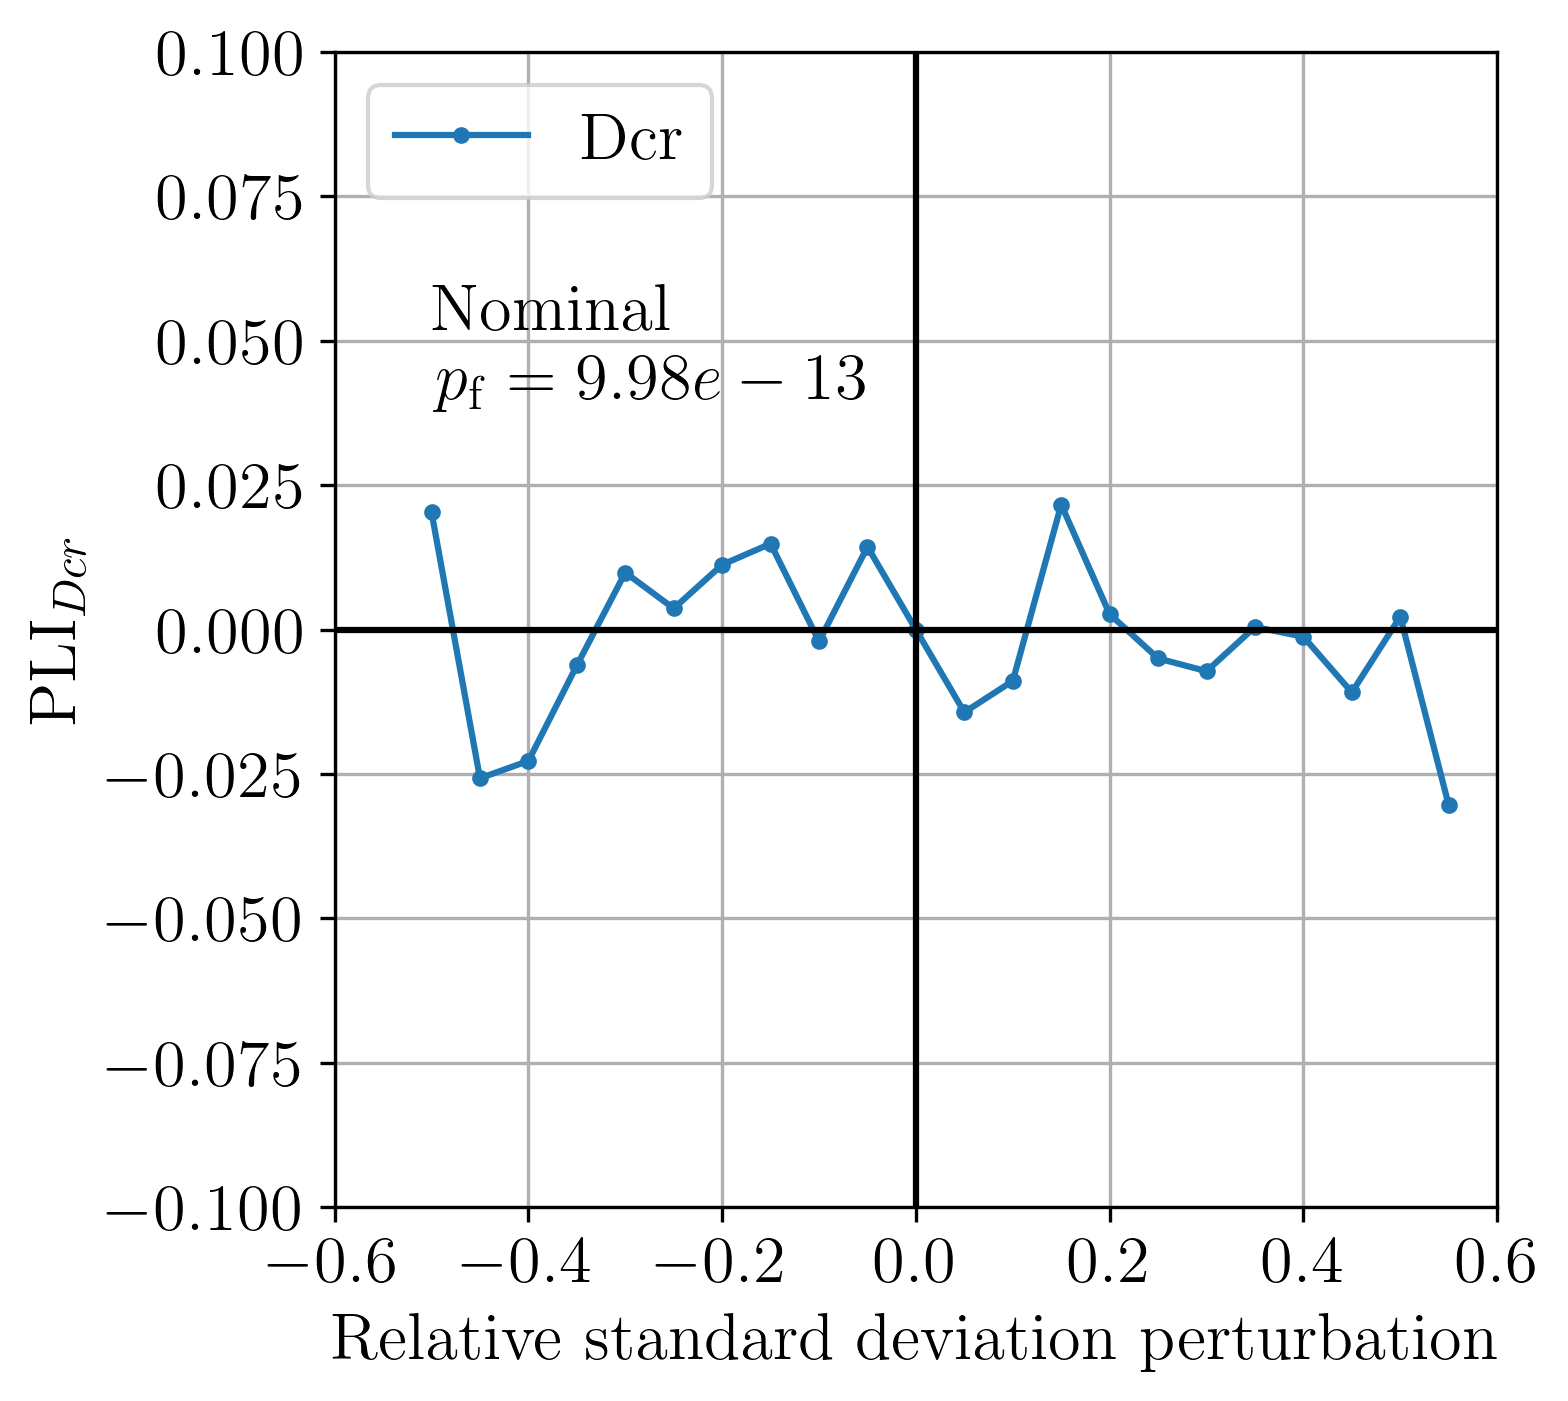
\includegraphics[width=\linewidth]{./part3/figures/OWT/PLI_Dcr_Hyp_LogNormal.png}
        \caption{Todo.}
    \end{subfigure}
    \begin{subfigure}[t]{0.45\linewidth}
        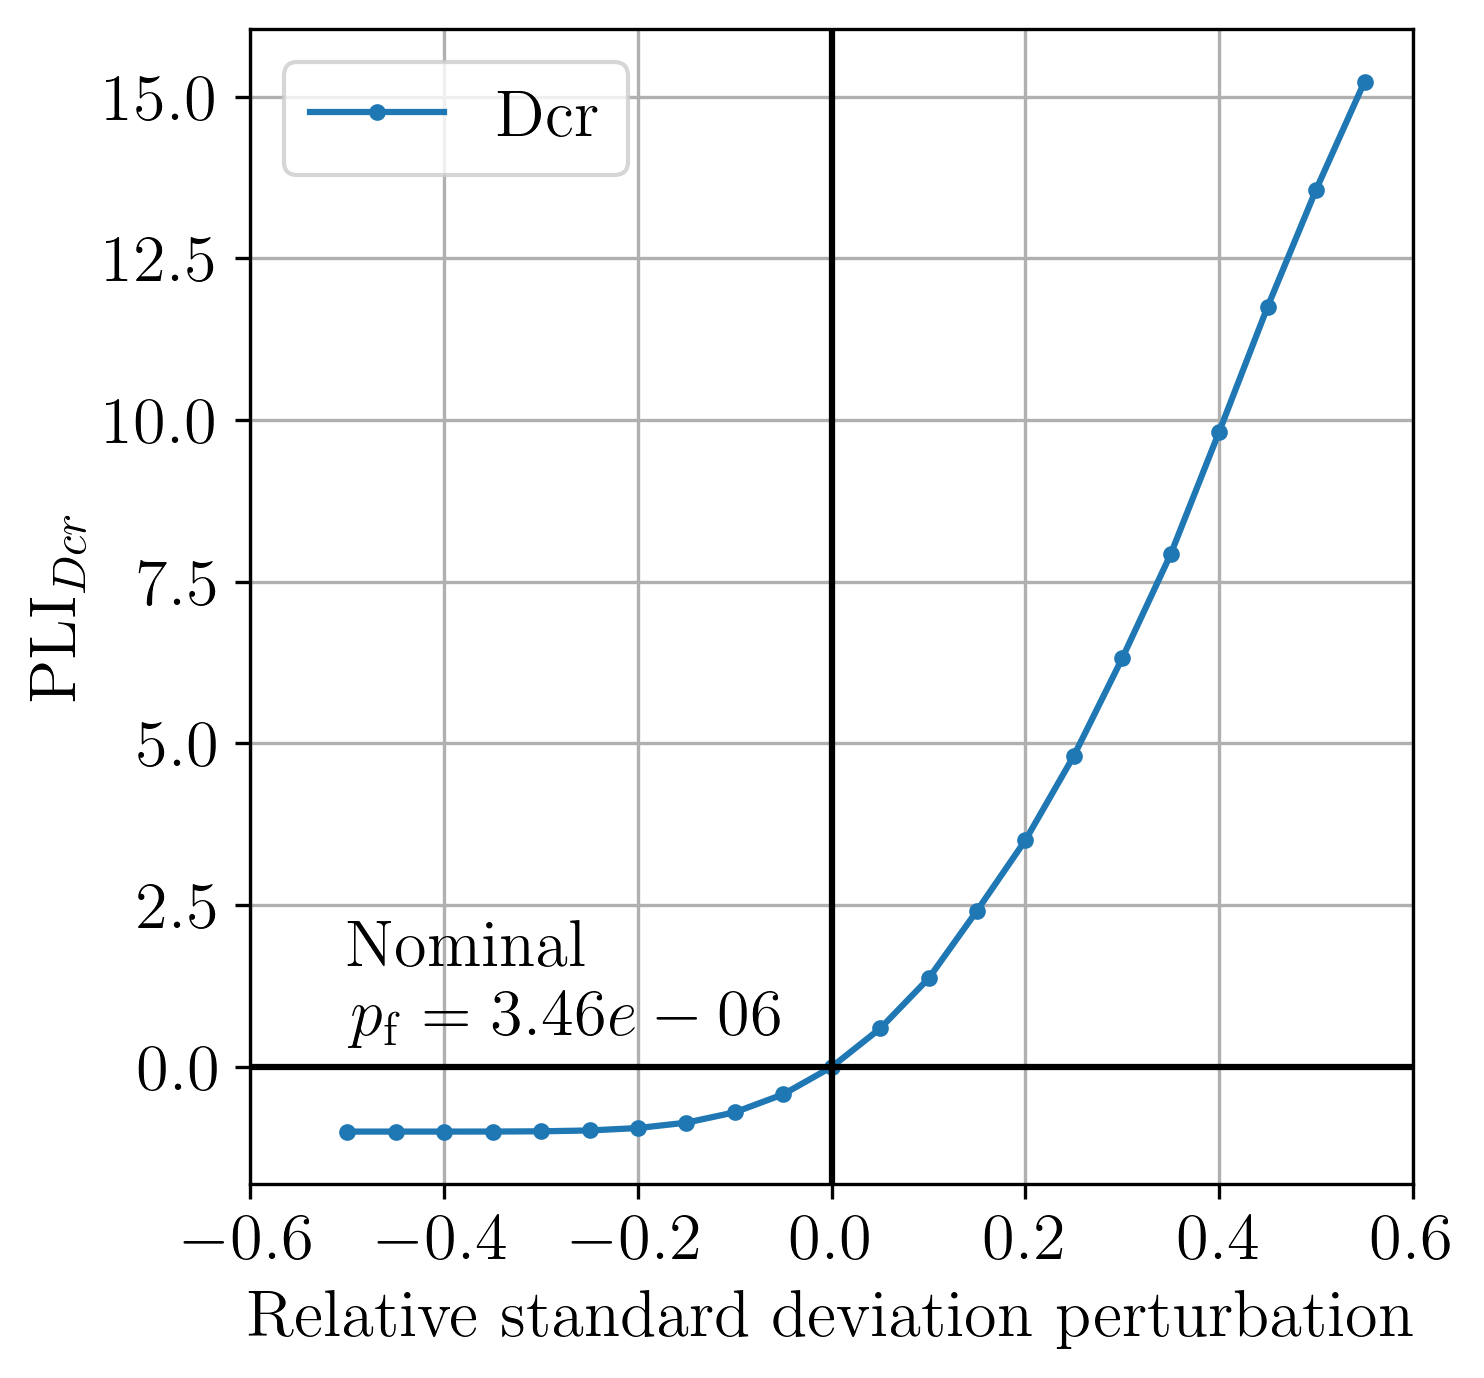
\includegraphics[width=\linewidth]{./part3/figures/OWT/PLI_Dcr_Hyp_Normal.png}
        \caption{Todo.}
    \end{subfigure}
    \label{fig:pli_resistance}
    \caption{Todo.}
\end{figure}

%============================================================%
%============================================================%
\section{Conclusion}
%============================================================%
%============================================================%




